\chapter{Redes Neuronales y Deep Learning}
\label{chapter:redes-neuronales-deep-learning}

En este capítulo vamos a dar un repaso a la teoría básica de Redes Neuronales y Deep Learning antes de entrar en la práctica. Repasaremos los fundamentos del aprendizaje con Redes Neuronales, veremos las estructuras de Aprendizaje Profundo o Deep Learning así como las capas de dichas redes que emplearemos en la práctica. Por último veremos una estructura de red que será utilizada en algunos de los modelos, los Autoencoders.

Para la elaboración de este capítulo nos basaremos en los libros de Bengio \cite{goodfellow_deep_2016} y Zaccone \cite{giancarlo_deep_2017}.

\section{Aprendizaje de las Redes Neuronales}

No todas las redes que vamos a emplear en la parte práctica corresponden al modelo ``Feedforward'', ya que también vamos a elaborar redes neuronales con capas recurrentes, pero vamos a estudiar el comportamiento primero de estas redes para luego explicar las modificaciones que dichas arquitecturas añaden.

En primer lugar, llamamos a este tipo de redes prealimentadas o ``Feedforward'' en inglés, porque la información fluye siempre en un sentido, desde la entrada hasta la salida obtenida. En las redes denominadas como recurrentes este sentido de la información se revierte en algunos puntos, realimentando la red con la propia salida de algunas capas o de todas ellas.

La representación más común de una red neuronal profunda es a través de la composición de funciones. Supongamos que estamos aproximando la función $f*(x)$ con una función $f(x)$ construida mediante tres funciones distintas: $f^{(1)}, f^{(2)} \ y \ f^{(3)}$ en este mismo orden. Entonces la representación de la función $f$ quedaría como:

$$f(x) = f^{(3)}(f^{(2)}(f^{(1)}(x))),$$

donde $x$ es la entrada de la red neuronal o lo que es lo mismo, una instancia o varias de nuestro conjunto de datos. En este caso además decimos que $f^{(1)}$ es la primera capa de la red, $f^{(2)}$ la segunda capa, etcétera.

Este tipo de estructuras se llaman profundas al tener varias capas y por tanto varias funciones que, al componerlas, aproximarán la función objetivo que tenemos. Las capas que se encuentran entre la primera y la última, al no ser capas ``visibles'' desde el exterior de la red las denominamos capas ocultas.

Estas capas están compuestas de unidades que denominamos neuronas haciendo una equivalencia con el modelo biológico. Una neurona recibe un número de entradas fijado, por ejemplo $n$. Para cada una de las entradas que recibe va aprendiendo un peso $w$, que luego multiplicará a cada una de las entradas y sumará para obtener un valor ponderado. A este valor ponderado se le aplica una función de activación que nos convierte dicho valor al rango que nosotros queramos para nuestro problema. Por tanto, una neurona produce como salida la función de activación aplicada a una combinación lineal de las entradas que recibe.

\begin{figure}[H]
	\centering
	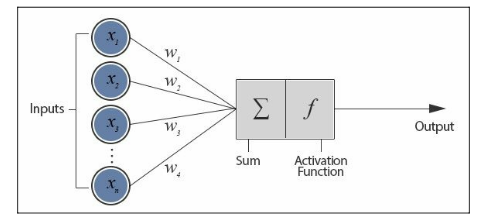
\includegraphics[scale=0.65]{imagenes/neurona.png}
	\caption{Representación de una neurona en una Red Neuronal.}
	\label{img:neurona}
\end{figure}

Como un detalle más a tener en cuenta, solemos añadir a las entradas una que denominamos como sesgo. Este sesgo es 1 y se suma a la combinación lineal, haciendo de término independiente en la ecuación de la recta que se está representando en el espacio de dominio de las instancias.

En cuanto a funciones de activación tenemos muchas sobre las que escoger, veamos las más comunes:

\begin{itemize}
	\item Rectified Linear Unit (ReLU): esta función de activación se define como 
	$$ReLU(x) = x^+ = max(0,x) \ , \ x\in \mathbb{R}^d,$$
	es decir, cero en los negativos y la función identidad en los positivos.
	\begin{figure}[H]
		\centering
		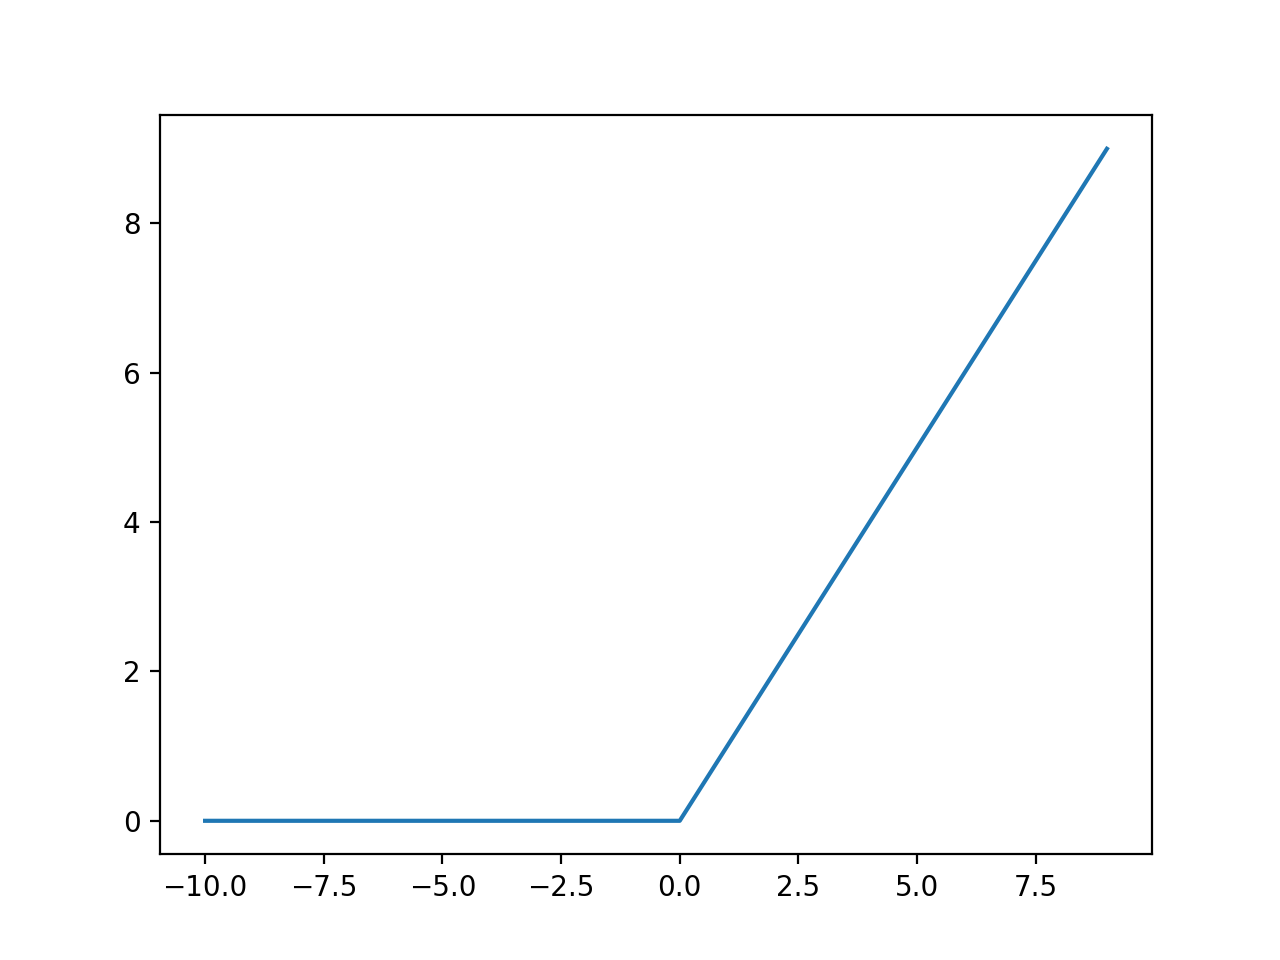
\includegraphics[scale=0.5]{imagenes/relu.png}
		\caption{Función ReLU.}
		\label{img:relu}
	\end{figure}
	\item Softmax: esta función de activación se define como:
	$$softmax : \mathbb{R}^d \rightarrow [0,1]^d$$
	$$softmax(x)_j = \frac{e^{x_j}}{\sum_{k=1}^{d}e^{x_k}}$$
	Con esta función se obtiene un valor con el mismo número de dimensiones que el que tuvieran los datos de entrada. Además, la salida se puede emplear para representar una distribución de probabilidad. Normalmente esta función de salida se emplea en problemas de clasificación donde vamos a obtener un valor entre 0 y 1 para cada una de las clases, siendo el mayor de estos la clase que el modelo predice.
	\item Sigmoide: esta función de activación se define como:
	$$sigmoide(x) = \frac{1}{1+e^{-x}}$$
	Esta función es una función real de variable real muy conocida y estudiada en matemáticas, con propiedades interesantes como que posee dos asíntotas horizontales y tiene una primera derivada no negativa.
	\begin{figure}[H]
		\centering
		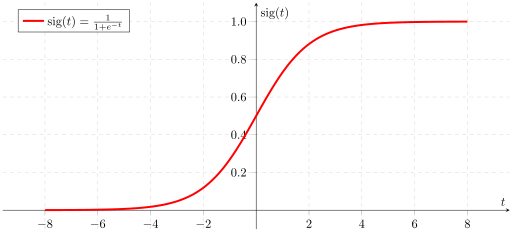
\includegraphics[scale=0.5]{imagenes/sigmoide.png}
		\caption{Función Sigmoide.}
		\label{img:sigmoide}
	\end{figure}
	Su valor máximo es $1$ y su valor mínimo es $0$.
	\item Tangente hiperbólica: la función tangente hiperbólica se define como:
	$$tanh : \mathbb{R}\rightarrow \mathbb{R} \ , \ tanh(x) = \frac{sinh(x)}{cosh(x)} = \frac{e^x - e^{-x}}{e^x + e^{-x}}$$
	\begin{figure}[H]
		\centering
		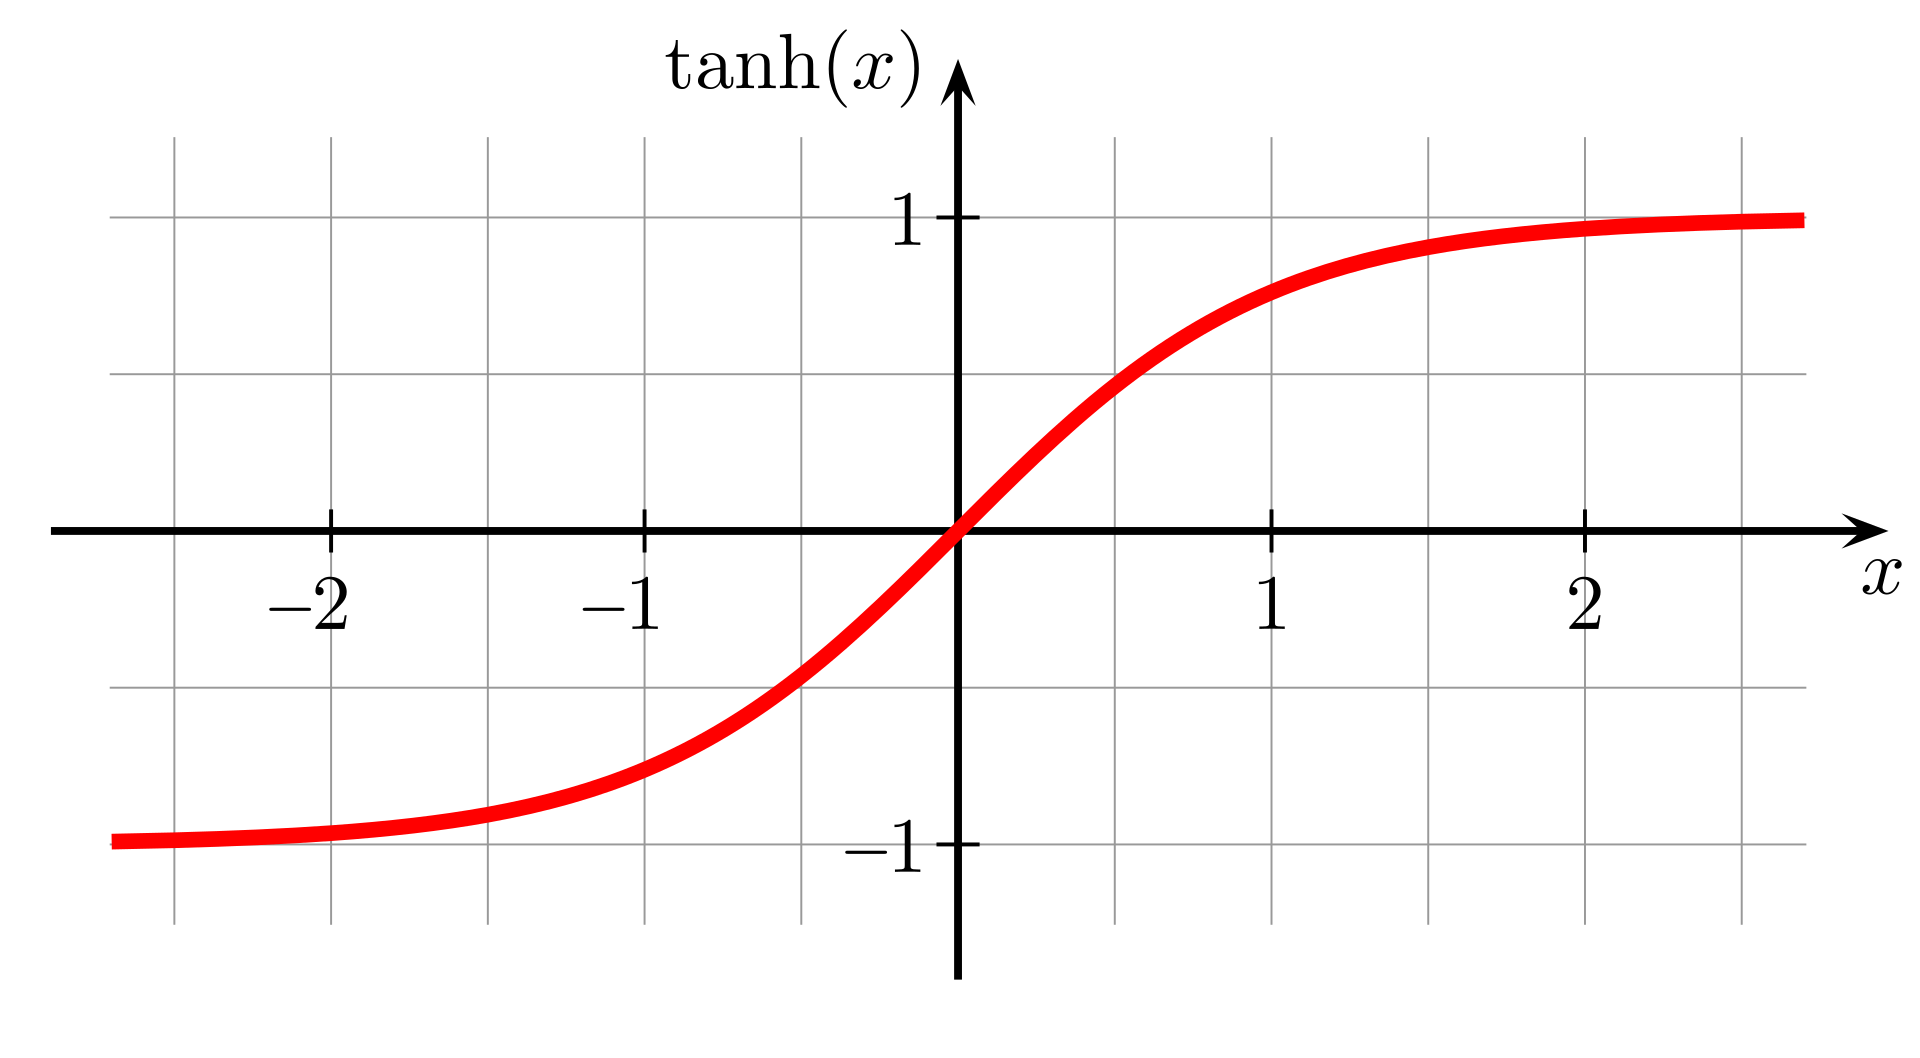
\includegraphics[scale=0.15]{imagenes/tangente_hiperbolica.png}
		\caption{Función tangente hiperbólica.}
		\label{img:tanh}
	\end{figure}
	Como podemos ver esta función de activación puede tomar valores en el intervalo $(-1,1)$.
\end{itemize}

Una vez que sabemos cuál es el comportamiento básico de una neurona vamos a ver cómo funciona el algoritmo empleado en el aprendizaje de las redes: Backpropagation.

Si describimos el proceso de forma sencilla podemos resumirlo en 4 pasos:

\begin{enumerate}
	\item Inicializar la red con pesos aleatorios.
	\item Calcular el error cometido en la predicción con los pesos actuales (pasada hacia delante) y, para cada una de las capas, ir volviendo hacia atrás desde la salida hasta la entrada.
	\item Enseñarle a la red el valor que debía predecir.
	\item Modificar los pesos en cada capa para mejorar la predicción.
\end{enumerate}

Lo primero que tenemos que hacer es definir las funciones de coste. Cuando estamos entrenando una red neuronal queremos tener una función de coste que optimizar, como hemos visto antes en la sección de Machine Learning. En este sentido podemos emplear varias funciones de coste en función de nuestras necesidades, pero es importante tener en cuenta que vamos a necesitar una para el proceso de aprendizaje.

En los cuatro pasos que hemos descrito, tras la inicialización de los pesos, tenemos el paso de la propagación hacia delante. Podemos ver este paso descrito en pseudocódigo en el algoritmo \ref{alg:forward-propagation}.

\begin{algorithm}[]{\Large{\textbf{Propagación hacia delante}}}
	
	\vspace{10px}
	
	\caption{Propagación hacia delante}
	\label{alg:forward-propagation}
	\KwIn{Profundidad de la red $l$}
	\KwIn{Matriz de pesos para la capa i-ésima $W^{(i)}$}
	\KwIn{Vector de sesgos de la capa i-ésima $b^{(i)}$}
	\KwIn{Instancia a procesar $x$}
	\KwIn{Salida objetivo $y^*$}
	\KwIn{Función de activación $g$}
	\KwIn{Función de similitud $L$}
	\KwIn{Función de regularización $\Omega$}
	\KwIn{Parámetros del modelo $\theta$}
	\KwIn{Ponderación de la regularización $\lambda$}
	
	\vspace{10px}
	
	$h^{(0)}\leftarrow x$
	
	\For{$k=1,...,l$}{
		
		$z^{(k)}\leftarrow W^{(k)}h^{(k-1)} + b^{(k)}$
		
		$h^{(k)}\leftarrow g(z^{(k)})$
		
	}

	$y\leftarrow h^{(l)}$
	
	$J\leftarrow L(y,y^*) + \lambda \Omega (\theta)$
	
	\vspace{10px}
	
	\KwOut{Predicción hecha $y$}
	\KwOut{Error cometido $J$}
	
	\vspace{5px}
\end{algorithm}

Como podemos ver, este algoritmo se encarga de ir pasando la información desde la entrada (la propia instancia) por cada una de las capas, multiplicando por su peso correspondiente, sumando el sesgo y aplicando la función de activación hasta que obtenemos una salida final.

Hemos visto en las secciones de Machine Learning que, una forma de hacer que nuestros algoritmos aprendan, es necesario obtener el gradiente del error para poder avanzar en el aprendizaje. Para realizar esta labor tenemos el algoritmo Backpropagation, que nos ayudará a calcular dicho gradiente de forma eficiente. Pensemos que tenemos que calcular el gradiente del modelo derivando con respecto a todos los parámetros. Cuando hablamos de Deep Learning es común tener muchas capas ocultas con un número elevado de neuronas, lo que aumenta muchísimo el número de parámetros y por tanto la complejidad del cálculo del gradiente.

Vamos a poner un ejemplo para poder ver la complejidad del cálculo del gradiente:

\begin{figure}[H]
	\centering
	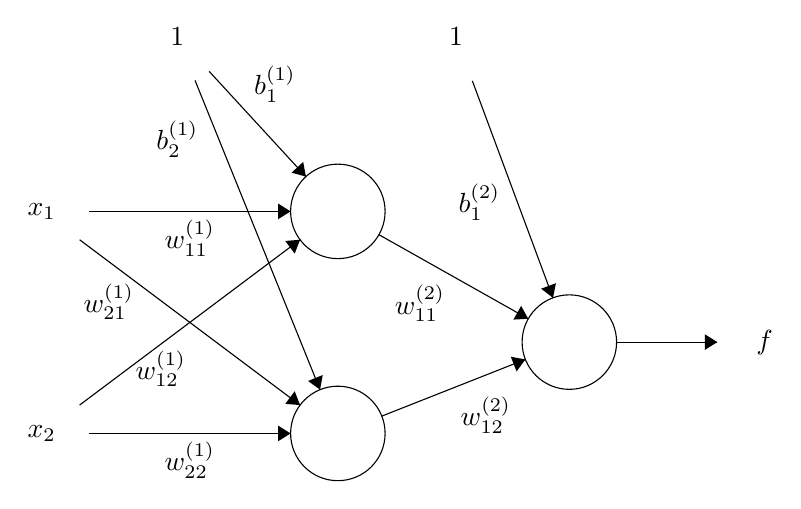
\begin{tikzpicture}[scale=0.2]
		\tikzstyle{every node}+=[inner sep=0pt]
		\draw [black] (34,-24.7) circle (3);
		\draw [black] (34,-38.8) circle (3);
		\draw [black] (48.7,-33) circle (3);
		\draw (15.2,-24.7) node {$x_1$};
		\draw (15.2,-38.8) node {$x_2$};
		\draw (61.1,-33) node {$f$};
		\draw (23.8,-13.6) node {$1$};
		\draw (41.5,-13.6) node {$1$};
		\draw [black] (36.79,-37.7) -- (45.91,-34.1);
		\fill [black] (45.91,-34.1) -- (44.98,-33.93) -- (45.35,-34.86);
		\draw (43.4,-36.44) node [below] {$w_{12}^{(2)}$};
		\draw [black] (36.61,-26.18) -- (46.09,-31.52);
		\fill [black] (46.09,-31.52) -- (45.64,-30.7) -- (45.15,-31.57);
		\draw (39.21,-29.35) node [below] {$w_{11}^{(2)}$};
		\draw [black] (17.6,-26.5) -- (31.6,-37);
		\fill [black] (31.6,-37) -- (31.26,-36.12) -- (30.66,-36.92);
		\draw (19.45,-29.25) node [below] {$w_{21}^{(1)}$};
		\draw [black] (17.6,-37) -- (31.6,-26.5);
		\fill [black] (31.6,-26.5) -- (30.66,-26.58) -- (31.26,-27.38);
		\draw (22.75,-33.50) node [below] {$w_{12}^{(1)}$};
		\draw [black] (51.7,-33) -- (58.1,-33);
		\fill [black] (58.1,-33) -- (57.3,-32.5) -- (57.3,-33.5);
		\draw [black] (25.83,-15.81) -- (31.97,-22.49);
		\fill [black] (31.97,-22.49) -- (31.8,-21.56) -- (31.06,-22.24);
		\draw (31.36,-16.61) node [left] {$b_1^{(1)}$};
		\draw [black] (42.54,-16.41) -- (47.66,-30.19);
		\fill [black] (47.66,-30.19) -- (47.85,-29.26) -- (46.91,-29.61);
		\draw (44.34,-24.11) node [left] {$b_1^{(2)}$};
		\draw [black] (24.93,-16.38) -- (32.87,-36.02);
		\fill [black] (32.87,-36.02) -- (33.04,-35.09) -- (32.11,-35.47);
		\draw (25.16,-20.1) node [left] {$b_2^{(1)}$};
		\draw [black] (18.2,-24.7) -- (31,-24.7);
		\fill [black] (31,-24.7) -- (30.2,-24.2) -- (30.2,-25.2);
		\draw (24.6,-25.2) node [below] {$w_{11}^{(1)}$};
		\draw [black] (18.2,-38.8) -- (31,-38.8);
		\fill [black] (31,-38.8) -- (30.2,-38.3) -- (30.2,-39.3);
		\draw (24.6,-39.3) node [below] {$w_{22}^{(1)}$};
	\end{tikzpicture}
	\caption{Ejemplo de una red neuronal sencilla.}
	\label{fig:backpropagation-ejemplo}
\end{figure}

Aquí podemos ver una red neuronal con 2 entradas y dos capas. Cada una de las capas tiene sus pesos y sus sesgos correspondientes. Entonces, en el modelo que hemos puesto como ejemplo, tenemos el siguiente vector de parámetros que determina nuestra red neuronal:

$$\theta = \Big(w_{11}^{(1)}, w_{12}^{(1)}, w_{21}^{(1)}, w_{22}^{(1)}, b_1^{(1)}, b_2^{(1)}, w_{11}^{(2)}, w_{12}^{(2)}, b_1^{(2)}\Big)$$

Con estos parámetros, la expresión de la salida de la red neuronal es:

$$f(x_1 , x_2 ; \theta) = g(w_{11}^{(2)}g(w_{11}^{(1)}x_1 + w_{12}^{(1)}x_2 + b_1^{(1)}) + w_{12}^{(2)}g(w_{21}^{(1)}x_1 + w_{22}^{(1)}x_2 + b_2^{(1)}) + b_1^{(2)})$$

Para simplificar las expresiones de las parciales vamos a notar lo siguiente:

$$\alpha = g' (w_{11}^{(2)}g(w_{11}^{(1)}x_1 + w_{12}^{(1)}x_2 + b_1^{(1)}) + w_{12}^{(2)} g(w_{21}^{(1)}x_1 + w_{22}^{(1)}x_2 + b_2^{(1)}) + b_1^{(2)}),$$

$$\beta =  g'(w_{11}^{(1)}x_1 + w_{12}^{(1)}x_2 + b_1^{(1)}) \ y$$

$$\gamma =  g'(w_{21}^{(1)}x_1 + w_{22}^{(1)}x_2 + b_2^{(1)}).$$

Con esto, podemos sacar las parciales de f, que nos van a ser necesarias en el cálculo del gradiente del coste J.

\footnotesize
\begin{alignat*}{3}
\frac{\partial f}{\partial w_{11}^{(1)}}(x_1,x_2;\theta)&=\alpha w_{11}^{(2)}\beta x_1,\quad&
\frac{\partial f}{\partial w_{12}^{(1)}}(x_1,x_2;\theta)&=\alpha w_{11}^{(2)}\beta x_2,\\
\frac{\partial f}{\partial w_{21}^{(1)}}(x_1,x_2;\theta)&=\alpha w_{12}^{(2)}\gamma x_1,\quad&
\frac{\partial f}{\partial w_{22}^{(1)}}(x_1,x_2;\theta)&=\alpha w_{12}^{(2)}\gamma x_2,\\
\frac{\partial f}{\partial b_{1}^{(1)}}(x_1,x_2;\theta)&=\alpha w_{11}^{(2)}\beta, \quad&
\frac{\partial f}{\partial b_{2}^{(1)}}(x_1,x_2;\theta)&=\alpha w_{12}^{(2)}\gamma, \\
\frac{\partial f}{\partial w_{11}^{(2)}}(x_1,x_2;\theta)&=\alpha g(w_{11}^{(1)}x_{1}+w_{12}^{(1)}x_2 + b_1^{(1)}),&&\\
\frac{\partial f}{\partial w_{12}^{(2)}}(x_1,x_2;\theta)&=\alpha g(w_{21}^{(1)}x_{1}+w_{22}^{(1)}x_2 + b_2^{(1)}),&\quad
\frac{\partial f}{\partial b_{1}^{(2)}}(x_1,x_2;\theta)&=\alpha.
\end{alignat*}
\normalsize

Viendo las expresiones que tenemos de las derivadas parciales se puede entender mejor la necesidad de eficiencia. En primer lugar, podemos ver que no tenemos una red para nada grande y ya tenemos que calcular 9 derivadas parciales. Por otro lado, podemos ver que hay términos que se repiten bastante con lo que, calculando primero estos términos, simplificamos la complejidad computacional de este problema.

Veamos el algoritmo de Backpropagation en pseudocódigo:

\begin{algorithm}[H]{\Large{\textbf{Propagación hacia atrás}}}
	
	\vspace{15px}
	
	\caption{Propagación hacia atrás}
	\label{alg:backpropagation}
	
	\vspace{10px}
	
	Calculamos el gradiente de la capa de salida.
	
	$d\leftarrow \nabla_y J(y,y^*;\theta) = \nabla_y L(y,y^*)$
	
	\For{$k=l,...,1$}{
	
		Aplicamos la regla de la cadena ($\odot$ es el producto componente a componente).
		
		$d\leftarrow \nabla_{z^{(k)}} J = d\odot g' (z^{(k)})$
		
		Calculamos los gradientes en los pesos y sesgos añadiendo también la regularización si la hubiera.
		
		$\nabla_{b^{(k)}}J = d + \lambda \nabla_{b^{(k)}} \Omega (\theta)$
		
		$\nabla_{W^{(k)}}J = d(h^{(k-1)})^T + \lambda \nabla_{W^{(k)}} \Omega (\theta)$
		
		$d\leftarrow \nabla_{h^(k-1)} J = \Big( W^{(k)} \Big)^T d$

	}
	
	\KwOut{Valor final del gradiente $d$}
	
	\vspace{5px}
\end{algorithm}

Como podemos ver, este algoritmo simplemente aplica la regla de la cadena y va calculando los gradientes sin repetir las derivadas capa a capa. Esta aproximación hace que el cálculo sea más sencillo y no se repita.

Llegados a este punto ya tenemos la salida que nos produce nuestra red neuronal con el algoritmo de propagación hacia delante y tenemos el cálculo del gradiente con la propagación hacia atrás. Ahora nos queda optimizar dicho coste con las herramientas que tenemos, es decir, resolver el problema de optimización que tenemos con el gradiente. 

Para resolver este problema tenemos la aproximación clásica de Gradiente Descendente Estocástico aunque no es la única herramienta que podemos usar para esto. Veremos algunas de las más utilizadas y cómo nos ayudan para obtener nuevos parámetros que mejoren el desempeño de las redes.

En primer lugar cabe explicar el algoritmo más empleado en esta tarea: Gradiente Descendente Estocástico. En Deep Learning se emplea el entrenamiento por lotes o batches en inglés, lo que hace inviable el uso de técnicas como Gradiente Descendente. Es por ello que se suele emplear la aproximación estocástica de Gradiente Descendente al ir calculando una aproximación del gradiente con números pequeños de muestras. Veamos el algoritmo en pseudocódigo:

\begin{algorithm}[H]{\Large{\textbf{Gradiente Descendente Estocástico en la iteración k-ésima}}}
	
	\vspace{15px}
	
	\caption{Gradiente Descendente Estocástico}
	\label{alg:sgd}
	\KwIn{Tasa de Aprendizaje $\epsilon_k$}
	\KwIn{Parámetros iniciales $\theta$}
	\KwIn{Tamaño de los lotes de datos $m$}
	
	\vspace{10px}
	
	\While{no se cumpla el criterio de parada}{
	
		Escoger un batch de datos de tamaño $m$ $x^{(1)}, ..., x^{(m)}$ con correspondientes objetivos $y^{(1)}, ..., y^{(m)}$
		
		Calculamos una estimación del gradiente.
		
		$\hat{g} \leftarrow \frac{1}{m}\nabla \sum_{i} L(f(x^{(i)};\theta), y^{(i)})$
		
		Actualizamos los parámetros.
		
		$\theta \leftarrow \theta - \epsilon_k \hat{g}$
	
	}
	
	\vspace{10px}
	
	\KwOut{Nuevos parámetros $\theta$}
	
	\vspace{5px}
\end{algorithm}

Como podemos ver, lo que estamos haciendo a cada paso es mejorar los parámetros del modelo en función del gradiente del coste, o más bien en este caso una aproximación del gradiente del coste. 

Con esto ya si tenemos el algoritmo completo: propagación hacia delante para obtener la salida predicha y el error, propagación hacia atrás para obtener el gradiente del coste y Gradiente Descendente Estocástico (u otro método) para optimizar los parámetros del modelo (o lo que es lo mismo, los pesos) hacia el mejor resultado.

También es común emplear variaciones de este algoritmo, pues puede mejorar con respecto a SGD aunque depende siempre del problema y los datos asociados. Las variaciones más comunes de este algoritmo son:

\begin{itemize}
	\item SGD con momento: a veces el algoritmo de Gradiente Descendente y el algoritmo de Gradiente Descendente Estocástico presentan una oscilación alrededor del mínimo de la función que pretenden minimizar. Veamos un ejemplo de esto:
	
	\begin{figure}[H]
		\centering
		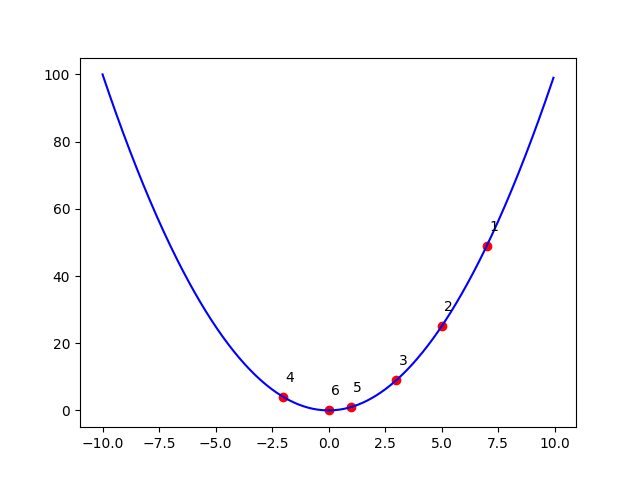
\includegraphics[scale=0.7]{imagenes/sgd.png}
		\caption{Oscilación alrededor del mínimo.}
		\label{img:oscilacion-sgd}
	\end{figure}

	En esta figura podemos ver cómo se produce una oscilación alrededor del mínimo. En funciones más complejas esta oscilación puede ser aún mayor y condicionar el funcionamiento del algoritmo de optimización. Esta variante del algoritmo hace que este zigzagueo u oscilación sea más leve, veamos el algoritmo en pseudocódigo:
	
	\begin{algorithm}[H]{\Large{\textbf{Gradiente Descendente Estocástico con momento}}}
		
		\vspace{15px}
		
		\caption{Gradiente Descendente Estocástico con momento}
		\label{alg:sgd-momento}
		\KwIn{Tasa de Aprendizaje $\epsilon$}
		\KwIn{Parámetros iniciales $\theta$}
		\KwIn{Tamaño de los lotes de datos $m$}
		\KwIn{Momento $\alpha$}
		\KwIn{Velocidad inicial $v$}
		
		\vspace{10px}
		
		\While{no se cumpla el criterio de parada}{
			
			Escoger un batch de datos de tamaño $m$ $x^{(1)}, ..., x^{(m)}$ con correspondientes objetivos $y^{(1)}, ..., y^{(m)}$
			
			Calculamos una estimación del gradiente.
			
			$\hat{g} \leftarrow \frac{1}{m}\nabla \sum_{i} L(f(x^{(i)};\theta), y^{(i)})$
			
			Actualizamos la velocidad.
			
			$v\leftarrow \alpha v - \epsilon \hat{g}$
			
			Actualizamos los parámetros.
			
			$\theta \leftarrow \theta + v$
			
		}
		
		\vspace{10px}
		
		\KwOut{Nuevos parámetros $\theta$}
		
		\vspace{5px}
	\end{algorithm}

	\item AdaGrad: esta es una versión adaptativa de SGD. El algoritmo varía los parámetros de forma inversamente proporcional a la raíz cuadrada de la suma de los cuadrados de los valores anteriores. Es decir, actualiza la tasa de aprendizaje decrementándola más rápido cuanto mayores sean las derivadas parciales. Como consecuencia de esto el avance en el espacio es más rápido que SGD. Veamos el pseudocódigo:
	
	\begin{algorithm}[H]{\Large{\textbf{Adagrad}}}
		
		\vspace{15px}
		
		\caption{Adagrad}
		\label{alg:adagrad}
		\textbf{Notación:} $\odot$ nota el producto componente a componente, $\sqrt{\cdot}$ es la raíz cuadrada componente a componente y las divisiones correspondientes son componente a componente.
		
		\KwIn{Tasa de Aprendizaje $\epsilon$}
		\KwIn{Parámetros iniciales $\theta$}
		\KwIn{Tamaño de los lotes de datos $m$}
		\KwIn{Constante inicial $\delta$ pequeña}
		
		\vspace{10px}
		
		$r\leftarrow 0$
		
		\While{no se cumpla el criterio de parada}{
		
			Escoger un batch de datos de tamaño $m$ $x^{(1)}, ..., x^{(m)}$ con correspondientes objetivos $y^{(1)}, ..., y^{(m)}$
			
			Calculamos una estimación del gradiente.
			
			$\hat{g} \leftarrow \frac{1}{m}\nabla \sum_{i} L(f(x^{(i)};\theta), y^{(i)})$
			
			$r\leftarrow r + \hat{g}\odot \hat{g}$
			
			$\Delta \theta \leftarrow - \frac{\epsilon}{\delta + \sqrt{r}} \odot \hat{g}$
			
			$\theta \leftarrow \theta + \Delta \theta$

		}
		
		\vspace{10px}
		
		\KwOut{Nuevos parámetros $\theta$}
		
		\vspace{5px}
	\end{algorithm}

	\item RMSProp: en vez de ir acumulando los gradientes se hace una media exponencial, lo que teóricamente mejor el comportamiento al minimizar funciones no convexas (aquellas idóneas para SGD).
	
	\begin{algorithm}[H]{\Large{\textbf{RMSProp}}}
		
		\vspace{15px}
		
		\caption{RMSProp}
		\label{alg:rmsprop}
		\textbf{Notación:} $\odot$ nota el producto componente a componente, $\sqrt{\cdot}$ es la raíz cuadrada componente a componente y las divisiones correspondientes son componente a componente.
		
		\KwIn{Tasa de Aprendizaje $\epsilon$}
		\KwIn{Parámetros iniciales $\theta$}
		\KwIn{Tamaño de los lotes de datos $m$}
		\KwIn{Constante inicial $\delta$ pequeña}
		\KwIn{Tasa de decaimiento $\rho$}
		
		\vspace{10px}
		
		$r\leftarrow 0$
		
		\While{no se cumpla el criterio de parada}{
			
			Escoger un batch de datos de tamaño $m$ $x^{(1)}, ..., x^{(m)}$ con correspondientes objetivos $y^{(1)}, ..., y^{(m)}$
			
			Calculamos una estimación del gradiente.
			
			$\hat{g} \leftarrow \frac{1}{m}\nabla \sum_{i} L(f(x^{(i)};\theta), y^{(i)})$
			
			$r\leftarrow \rho r + (1-\rho)\hat{g}\odot \hat{g}$
			
			$\Delta \theta \leftarrow - \frac{\epsilon}{\delta + \sqrt{r}} \odot \hat{g}$
			
			$\theta \leftarrow \theta + \Delta \theta$
			
		}
		
		\vspace{10px}
		
		\KwOut{Nuevos parámetros $\theta$}
		
		\vspace{5px}
	\end{algorithm}

	\item Adam: es una modificación de RMSProp con momento. Veamos el pseudocódigo:
	
	\begin{algorithm}[H]{\Large{\textbf{Adam}}}
		
		\vspace{15px}
		
		\caption{Adam}
		\label{alg:Adam}
		\textbf{Notación:} $\odot$ nota el producto componente a componente, $\sqrt{\cdot}$ es la raíz cuadrada componente a componente y las divisiones correspondientes son componente a componente.
		
		\KwIn{Tasa de Aprendizaje $\epsilon$}
		\KwIn{Parámetros iniciales $\theta$}
		\KwIn{Tamaño de los lotes de datos $m$}
		\KwIn{Constante inicial $\delta$ pequeña}
		\KwIn{Tasas de decaimiento $\rho_1 , \rho_2 \in [0,1)$}
		
		\vspace{10px}
		
		$s\leftarrow 0$
		
		$r\leftarrow 0$
		
		$t\leftarrow 0$
		
		\While{no se cumpla el criterio de parada}{
			
			Escoger un batch de datos de tamaño $m$ $x^{(1)}, ..., x^{(m)}$ con correspondientes objetivos $y^{(1)}, ..., y^{(m)}$
			
			Calculamos una estimación del gradiente.
			
			$\hat{g} \leftarrow \frac{1}{m}\nabla \sum_{i} L(f(x^{(i)};\theta), y^{(i)})$
			
			$t\leftarrow t+1$
			
			$s\leftarrow \rho_1 \cdot s + (1-\rho_1)\hat{g}$
			
			$r\leftarrow \rho_2 \cdot s + (1-\rho_2)\hat{g}\odot \hat{g}$
			
			$\hat{s}\leftarrow \frac{s}{1-\rho_1^r}$
			
			$\hat{r}\leftarrow \frac{r}{1-\rho_2^r}$
			
			$\Delta \theta \leftarrow - \frac{\epsilon}{\delta + \sqrt{\hat{r}}}\hat{s}$
			
			$\theta \leftarrow \theta + \Delta \theta$
			
		}
		
		\vspace{10px}
		
		\KwOut{Nuevos parámetros $\theta$}
		
		\vspace{5px}
	\end{algorithm}
\end{itemize}

Con esto ya hemos cubierto cómo aprende una red neuronal de forma completa.

\section{Capas empleadas}

\subsection{Capas densas o totalmente conectadas}

En las redes neuronales tenemos distintos tipos de capas o neuronas que podemos utilizar en la construcción de la arquitectura de la red. La estructura explicada con anterioridad asumía el uso de capas densas o totalmente conectadas. Estas capas tienen exactamente el comportamiento descrito en la figura \ref{img:neurona}. Debemos tener en cuenta que vamos a emplear un tipo de capa u otro en función de la información que queramos obtener de nuestros datos.

En primer lugar vamos a hacer un pequeño repaso de las capas densas o totalmente conectadas. Estas capas están ya descritas en la sección anterior, por lo que no nos vamos a detener más en esto. Las capas densas son empleadas cuando tenemos entradas de tipo numérico, ya sea una única entrada numérica o un vector de números. 

Lo más común es que esta capa siempre aparezca en la mayoría de estructuras de redes neuronales, pues aunque sea una red por ejemplo con mayoría de capas convolucionales, normalmente las últimas o las primeras son capas densas que nos permiten igualar la dimensión de los datos a lo que nosotros queramos (en función de si es un problema de predicción, regresión o clasificación u otro tipo).

El funcionamiento de este tipo de capas es muy sencillo. Tenemos una neurona que recibe tantas conexiones como neuronas o entradas hubiera en la capa anterior más un sesgo. Todas estas conexiones tienen un peso asignado como vimos en el ejemplo \ref{fig:backpropagation-ejemplo}. Este comportamiento se replica en toda la capa, es decir, todas las neuronas de la capa reciben como entrada todas estas conexiones con un valor numérico y un peso asignado. Estos pesos y valores se combinan de forma lineal, es decir, multiplicando cada valor numérico por cada uno de los pesos y sumándose. Tras la suma simplemente se añade el término de sesgo y se aplica a todo esto la función de activación, que es intrínseca de la capa. Esto quiere decir que, para que el funcionamiento de la capa sea homogéneo, se aplica la misma función de activación a todas las neuronas que componen dicha capa. Esto lo que nos va a producir como salida es un vector de valores numéricos, que son las salidas de cada una de las neuronas de nuestra capa.

\begin{figure}[H]
	\centering
	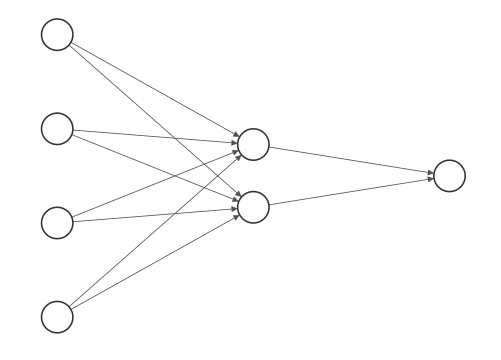
\includegraphics[scale=0.5]{imagenes/fcnn_example.png}
	\caption{Ejemplo de red neuronal con capas densas.}
	\label{img:ejemplo-fcnn}
\end{figure}

En este ejemplo podemos ver que tenemos 3 capas, una capa de entrada, una capa oculta y una de salida. La capa de entrada tiene 4 neuronas, por lo que recibe como entrada un vector numérico de 4 valores que se asocian cada uno con una neurona. La capa oculta tiene 2 neuronas que reciben como entrada cada una un vector numérico de 4 valores, produciendo dicha capa al final un vector de dos valores numéricos. Por último la capa de salida tiene una única neurona, por lo que la salida de la red es un único valor numérico, recibiendo como entrada un vector de dos valores.

Esta capa nos servirá en todas las estructuras Deep Learning elaboradas que emplearemos más tarde en la aplicación práctica.

\subsection{Capas convolucionales}

En esta sección vamos a explicar el funcionamiento de las capas de convolución, los datos que reciben y los datos que obtenemos a través de la operación de convolución.

Lo primero que tenemos que hacer es definir el operador de convolución para poder ver cómo y donde emplearlo en una red neuronal. Supongamos que tenemos una serie de datos que dependen de una variable $t$ temporal, es decir, por ejemplo podemos tener distintos valores de una serie temporal. Si la función que nos da dichos valores de la serie temporal es $x(t)$, podemos definir una función que suavice a $x(t)$ de la siguiente forma:

$$s(t) = \int x(a)\cdot w(t-a) da = (x * w)(t)$$

Donde $w(a)$ es una ponderación que hacemos a los valores de la función $x(t)$. Además, se suele notar esta operación con el asterisco como hemos hecho. Esta función suavizada de la original es lo que llamamos operación de convolución.

En un caso real de aplicación no vamos a tener la función $x(t)$ que nos da la salida u objetivo de nuestro problema en cada instante de tiempo, pues entonces no habría problema al estar resuelto y modelado. Por contra, lo que vamos a tener normalmente es una serie de valores de ejemplo de salida. Al ser este un número finito de muestras, sabemos que la integral se define como una suma y por tanto podemos definir el operador de convolución como:

$$s(t) = (x*w)(t) = \sum_{a=-\infty}^{\infty}x(a)w(t-a)$$

Está claro que esta definición que hemos dado no tiene sentido cuando tenemos más de un valor, es decir, cuando la función $x$ no es real, si no que da como salida un vector de números.

Normalmente empleamos como entrada en este tipo de redes con capas convolucionales un vector de datos, por ejemplo, una imagen o varias instancias de una serie temporal. Esto hace que tengamos como input una matriz bidimensional o tridimensional normalmente como entrada, por lo que tenemos que pensar en hacer la operación de convolución en varios ejes. La aplicación de esta operación nos va a dar como resultado de nuevo una matriz, como es natural. Por tanto, suponiendo que $I$ es nuestra imagen de entrada o grupo de datos de una serie temporal, podemos definir el operador de convolución sobre dos ejes como:

$$S(i,j) = (I*K)(i,j) = \sum_{m} \sum_{n} I(m,n)K(i-m,j-n)$$

Donde K es un núcleo o kernel de dos dimensiones, como la entrada, pero no tiene por qué tener el mismo tamaño que la misma. Como característica de esta operación tenemos que es conmutativa, es decir, $(I*K)(i,j) = (K*I)(i,j)$ al invertirse únicamente el producto que tenemos dentro de la sumatoria.

Veamos un ejemplo de como aplicamos esta operación de convolución a una matriz de dos dimensiones $3x4$ con un kernel $2x2$:

\begin{figure}[H]
	\centering
	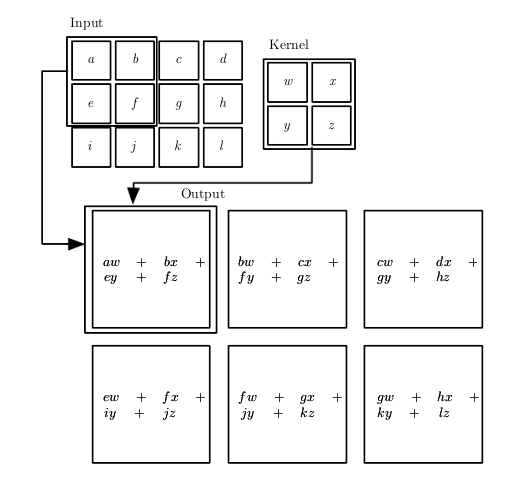
\includegraphics[scale=0.65]{imagenes/convolucion.png}
	\caption{Ejemplo de operación de convolución.}
	\label{img:convolucion}
\end{figure}

Como podemos ver, el resultado de esta operación es tomar el kernel e ir deslizándolo por la matriz para obtener, por cada una de estas posiciones, un valor real y construir de esta forma una matriz de salida. En este caso, con un kernel $2x2$ y con una matriz de entrada $3x4$ obtenemos una matriz de salida $2x3$.

Precisamente en este tipo de capas, los pesos son los núcleos que aplicamos en la operación de convolución, por lo que nuestro algoritmo de backpropagation se orientará en optimizar dichos valores.

Normalmente, una capa de convolución dentro de una red neuronal hace esta operación de convolución con varios filtros o kernels, por ejemplo 32, 64, 128 u otro número. Si elegimos tamaño de kernel $3x3$ entonces tendríamos 32, 64, 128 u otro número de matrices con 9 pesos en cada una que entrenaremos con backpropagation.

Con esta capa de convolución se suele combinar una capa u operador de Pooling o agrupación. Este operador nos va a servir para agrupar los datos y reducir la dimensión. El operador de agrupación se aplica a cada una de las salidas de la convolución, es decir, al resultado de hacer $(I*K)$ con cada uno de los núcleos. Podemos aplicar aquí por ejemplo un agrupamiento $2x2$ que nos reducirá la dimensión de la salida a la mitad para cada núcleo.

Esta operación, a parte de reducir la dimensión de la salida, nos va a ayudar a que nuestra salida sea más robusta. Pensemos por ejemplo en que tenemos imágenes como datos de entrada, si las imágenes de entrada varían ligeramente (una ligera traslación) entonces la operación de Pooling nos va a ayudar a que la información que extraemos sea invariante frente a estas pequeñas variaciones.

Las dos operaciones de agrupamiento que se suelen emplear en la capa de Pooling son el máximo y la media. Esto lo que hace es obtener como valor final la media o el máximo del tamaño de Pooling que estemos haciendo. Pensemos por ejemplo que la salida de la convolución es una matriz $8x8$ y nosotros hacemos un agrupamiento $2x2$. Entonces vamos a ir pasando por la salida una matriz $2x2$ y calculando la media o el máximo de dicha matriz para obtener un único valor, después desplazamos uno a la derecha y hacia abajo una unidad también cuando acabemos la fila completa. De esta forma iremos construyendo una matriz con los máximos o medias de la salida de la convolución.

Ya que entendemos un poco mejor cómo funciona la operación de convolución y cómo funcionan las capas convolucionales y de agrupamiento, vamos a repasar brevemente el objetivo y el uso de estas capas en la redes neuronales. 

Para poder aplicar la operación de convolución de forma coherente debemos tener datos que tengan una dependencia local, por ejemplo las imágenes o una serie temporal sobre la que agrupamos las instancias consecutivas en el tiempo para formar un vector (en el caso de una serie temporal real) o una matriz (en el caso de una serie temporal de varias variables de salida). 

Con la operación de convolución, al ir repitiéndola varias veces junto con el agrupamiento, obtenemos información local interesante e importante para nuestro problema. Por ejemplo sería algo común que, tras la aplicación de varias capas de convolución, obtuviéramos como salida de esos parches formas, objetos o secciones de imágenes que sean de relevancia para nuestra tarea final. Esto ocurre de igual forma con las series temporales u otro tipo de datos, pero es más sencillo explicar este fenómeno con las imágenes por la capacidad de visualizar los datos.

Por tanto estas capas no están pensadas para ser la última o primera capa de nuestra red, si no para formar parte de ella para obtener características de nuestros datos que nos ayuden en la tarea de predicción, regresión o clasificación que tengamos como objetivo.

\subsection{Capas recurrentes y LSTM}

Este tipo de redes y capas están pensadas precisamente para recibir como entrada varias instancias consecutivas en el tiempo de una serie temporal. Para poder hacer una red con un mejor desempeño en este tipo de datos, vamos a hacer que los pesos de una capa en un momento determinado de la serie temporal, puedan afectar a momentos posteriores y capas posteriores dependiendo de la estructura de la red. Con ello, la intención es poder sacar patrones que no dependan del tiempo y sean poco sensibles a variaciones como reflexiones de los datos (cambiar inicio por fin y fin por inicio) y procesar datos de distinto tamaño.

En este tipo de datos siempre tenemos una dependencia de los actuales con los anteriores en el tiempo, es decir, podemos describir el dato en el instante $t$ de tiempo a partir de los datos en los instantes anteriores. Supongamos que tenemos representado el estado del sistema como $s^{(t)}$ entonces esto se traduce en que:

$$s^{(t)} = f(s^{(t-1)};\theta),$$

es decir, el valor en el instante $t$ depende del $t-1$ y así sucesivamente. En una aplicación real de este tipo de redes, fijamos un número de pasos en el tiempo que vamos a analizar en bloque. Por tanto este proceso recurrente se puede desarrollar de forma extensiva. Si fuese con 3 pasos en el tiempo tendríamos que $s^{(3)}$ se podría expresar como:

$$s^{(3)} = f(s^{(2)};\theta) = f(f(s^{(1)};\theta);\theta)$$

Ahora vamos a hacer este ejemplo algo más real. Supongamos que tenemos nuestro sistema $h(t)$ (se nota con h porque será oculto dentro de la red, hidden) y una señal externa (la serie temporal) entonces podemos describir nuestro sistema dinámico recurrente como:

$$h^{(t)} = f(h^{(t-1)},x^{(t)};\theta)$$

Esta función que modela nuestro sistema con el estado del mismo y con una señal externa la podemos desenrollar, es decir, eliminar la componente recurrente al estar basado en un número finito de muestras como hemos hecho anteriormente.

\begin{figure}[H]
	\centering
	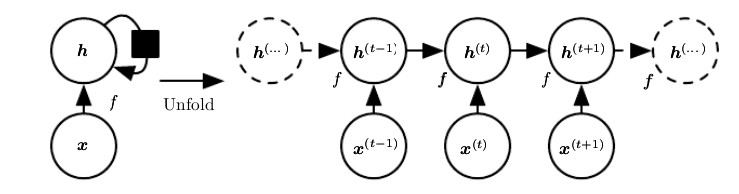
\includegraphics[scale=0.5]{imagenes/desenrollado.png}
	\caption{Desenrollado de la función recurrente.}
	\label{img:desenrollado-recurrente}
\end{figure}

Como podemos ver en el esquema, el estado anterior del sistema influye sobre el estado actual y la señal exterior actual influye también en el estado del sistema.

Con esta idea de compartir pesos y que el estado actual vaya dependiendo de los anteriores, llevando una dependencia temporal, podemos elaborar distintos tipos de redes neuronales.

\begin{figure}[H]
	\centering
	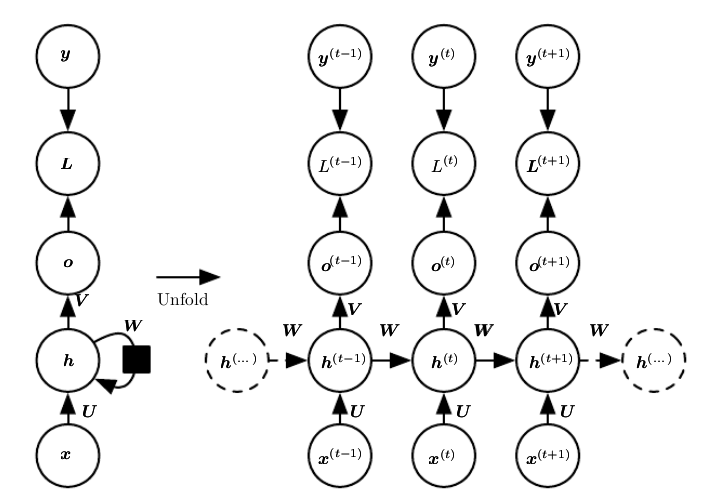
\includegraphics[scale=0.5]{imagenes/rnn1.png}
	\caption{Red recurrente que produce una salida en cada paso temporal con conexiones entre las unidades ocultas.}
	\label{img:red-recurrente1}
\end{figure}

En este caso vemos un esquema, en el que tenemos las entradas o estímulos externos que describíamos anteriormente, el estado interno del sistema representado con $h$, la salida producida $o$, la función de pérdida de la salida predicha frente a la real $L$ y la salida real $y$.

En este tipo de red neuronal tenemos la entrada ponderada por unos pesos $U$, el estado interno ponderado por pesos $W$ y la salida ponderada por pesos $V$. Podemos ver que esta estructura nos da, para cada unidad de tiempo, su salida correspondiente y  como podemos ver, los pesos de la capa oculta solo se usan de un instante de tiempo a otro de la misma capa oculta o estado del sistema.

\begin{figure}[H]
	\centering
	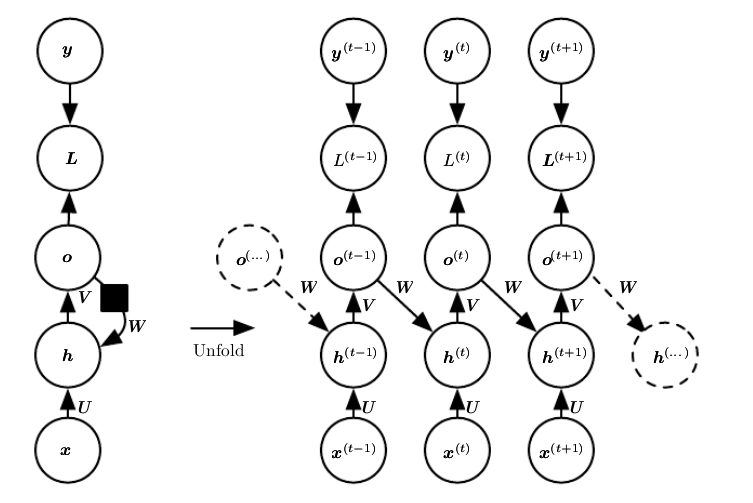
\includegraphics[scale=0.5]{imagenes/rnn2.png}
	\caption{Red recurrente que produce una salida en cada paso temporal con conexiones de la salida a las unidades ocultas.}
	\label{img:red-recurrente2}
\end{figure}

En este caso podemos ver como no hay conexiones de pesos entre las neuronas ocultas, si no de la salida anterior a la neurona del estado del sistema en el instante de tiempo siguiente. Esto nos está dando información de la salida anterior para condicionar la siguiente salida, de hecho es la única información que recibe el siguiente estado de tiempo de la red neuronal además de la señal externa.

\begin{figure}[H]
	\centering
	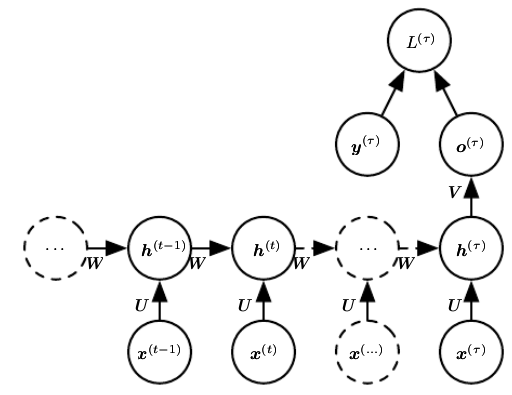
\includegraphics[scale=0.5]{imagenes/rnn3.png}
	\caption{Red recurrente que produce una única salida con conexiones entre las unidades ocultas.}
	\label{img:red-recurrente3}
\end{figure}

Como podemos ver, en este caso tenemos que los pesos se comparten sólo en la capa oculta. Esta red va almacenando conocimiento hasta llegar al último paso temporal, en el cual se emplea lo obtenido de los instantes de tiempo anteriores para producir una única salida. Este tipo de redes pueden usarse por ejemplo para predecir el siguiente valor de una serie temporal conociendo los valores de los instantes de tiempo anteriores.

Estos ejemplos que hemos dado no son una taxonomía, si no una serie de modelos que podemos utilizar y empleamos como ejemplo. Cada problema tiene unos requerimientos y objetivos que queremos cumplir y debemos ajustar nuestra red al problema que tengamos en consideración.

Hemos hecho un breve repaso de la idea de las redes neuronales recurrentes. En nuestro caso de aplicación práctica hemos empleado capas LSTM o Long-Short Term Memory, por lo que vamos a repasar cómo funcionan estas capas de forma teórica.

Las capas LSTM entran dentro de un tipo de redes neuronales recurrentes llamadas redes recurrentes con puertas. La idea es que estas redes elaboran caminos entre las entradas, salidas y estados internos que permiten recordar información u olvidarla si ya no nos es útil. Veamos esto con un esquema de cómo funcionan las LSTM:

\begin{figure}[H]
	\centering
	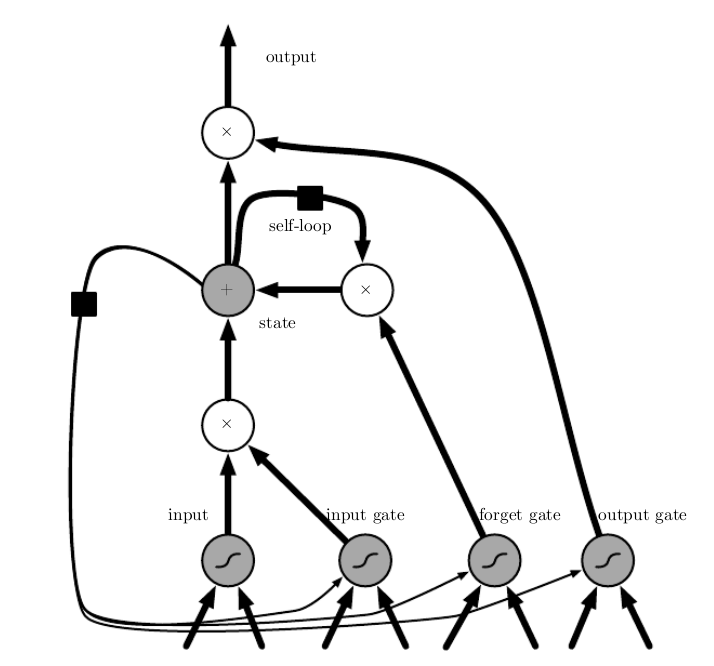
\includegraphics[scale=0.5]{imagenes/lstm.png}
	\caption{Esquema de funcionamiento de una celda LSTM.}
	\label{img:esquema-lstm}
\end{figure}

Estas celdas o neuronas están conectadas entre sí a través de los estados del sistema como en una red recurrente normal, por lo que cada uno de los estados tendría un peso y una conexión con la siguiente neurona. Podemos ver que la entrada se procesa con una neurona tradicional como teníamos en las capas densas, llegando esta entrada al estado de la celda y siendo acumulado o añadido si la función de activación y el resto de la celda lo permite. Podemos ver que el estado tiene un ciclo consigo mismo, moderado por la puerta de olvido. Esta puerta puede permitir olvidar el estado si se considera que es más beneficioso que conservarlo. El estado se realimenta de nuevo a la entrada tanto a la unidad de entrada, como a la de olvido y salida para poder tener su propio estado anterior como entrada del siguiente y decidir su acción. La neurona de salida puede cortar la salida producida por la celda.

Todo este esquema permite que la celda adquiera el estado de la anterior y lo integre como una entrada, procese su propia entrada basándose también en su estado anterior y decida si acumula el conocimiento, olvida o corta su salida en función de lo que mejor función de pérdida otorgue. Todo esto hace que nuestra celda pueda recordar todo el contenido de la serie temporal u olvidarlo en algún punto determinado u obviar una entrada si no se percibe de interés.

Este tipo de redes son actualmente muy exitosas en aplicación sobre texto, predicciones en series temporales y uso en vídeo para detección de trayectorias entre otros ejemplos. Nosotros las emplearemos en la parte práctica tanto solas como combinadas con convoluciones para obtener características algo mejores para alimentar la red.

\section{Autoencoders}

En la sección práctica veremos el uso de Autoencoders para la tarea de detección de anomalías que queremos desarrollar, por lo que necesitamos un poco de fundamento teórico para poder entender bien el funcionamiento de este tipo de arquitecturas.

El objetivo principal de estas arquitecturas es conseguir una codificación de los datos, es decir, una representación de los mismos en un espacio de menor dimensión que permita obtener suficiente información de ellos como para reconstruirlos a los originales cometiendo un error pequeño asumible. Esta arquitectura se puede ver dividida por tanto en dos partes, la función codificadora que codifica el dato y la función decodificadora que reconstruye el dato a partir de la codificación.

Normalmente no estamos interesados en la salida del Autoencoder, es decir en la decodificación del dato, si no en la codificación pero en nuestro caso estaremos interesados en la reconstrucción. Aunque nuestro objetivo sea obtener una salida final de calidad es fundamental fijarse en la codificación obtenida y que esta sea buena.

El tipo de Autoencoders que vamos a emplear son denominados como Autoencoders incompletos, ya que el objetivo es que la codificación sea de menor dimensión que la que poseen los datos originales. El proceso de aprendizaje de estos Autoencoders es sencillo: introducimos como entrada los datos originales y como salida predicha los mismos datos de entrada para que la red pueda aprender a reconstruirlos.

Para el proceso de detección de anomalías vamos a usar esta arquitectura del siguiente modo: entrenaremos con datos limpios sin anomalías e intentaremos que la reconstrucción sea lo más ajustada posible pero siempre con una codificación del menor tamaño posible para forzar la extracción de las características meramente esenciales. Tras esto lo que haremos será predecir, cuando obtengamos una reconstrucción con poco error estaremos ante un dato no anómalo o parecido a los no anómalos vistos previamente por la red y por tanto es capaz de reconstruirlos con poco error. Por contra si no es capaz de reconstruirlos bien y se comete mucho error estaremos ante un dato que no es normal y por tanto no ha sido visto por la red neuronal, cometiendo un mayor error de reconstrucción.

Veamos un ejemplo de un Autoencoder de capas totalmente conectadas:

\begin{figure}[H]
	\centering
	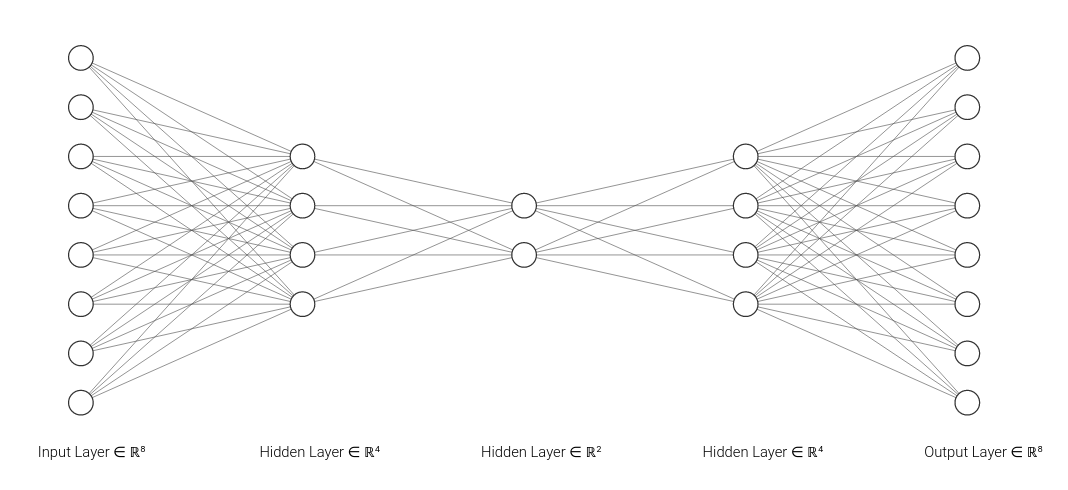
\includegraphics[scale=0.35]{imagenes/autoencoder_ejemplo.png}
	\caption{Ejemplo de Autoencoder con capas totalmente conectadas.}
	\label{img:ejemplo-autoencoder}
\end{figure}

Como podemos observar en la figura \ref{img:ejemplo-autoencoder} tenemos datos de entrada con 8 variables, reducimos primero la dimensión a 4 y finalmente la codificación reduce la dimensión a dos variables. Tras esto viene la decodificación que devuelve los datos primero a 4 variables y finalmente a las 8 iniciales.

Esta misma arquitectura se puede emplear con varias capas distintas, en la práctica nosotros emplearemos capas densas y capas LSTM para extraer una codificación de menor dimensionalidad que la original.